\documentclass[final]{beamer}

% ==============================================================================
% PACKAGES
% ==============================================================================
\usepackage[size=a0,orientation=landscape,scale=1.05]{beamerposter}
\usepackage[utf8]{inputenc}
\usepackage[T1]{fontenc}
\usepackage{lmodern}
\usepackage{graphicx}
\usepackage{booktabs}
\usepackage{multicol}
\usepackage{ragged2e}
\usepackage{xcolor}
\usepackage{microtype}
\usepackage{tikz}
\usetikzlibrary{calc, shadows.blur, shapes.symbols, patterns, decorations.pathmorphing}
\usepackage[most]{tcolorbox}

% ==============================================================================
% COLOR PALETTE (Solar & Data Theme)
% ==============================================================================
% Backgrounds
\definecolor{PageBG}{HTML}{F0F4F8}       % Very light blue-grey for page bg
\definecolor{BlockBG}{HTML}{FFFFFF}       % White for content boxes

% Primary Brand Colors
\definecolor{DeepSpace}{HTML}{0B1E3B}     % Dark Navy (Header/Footer)
\definecolor{SolarGold}{HTML}{FFB400}     % Active Sun color (Accents)
\definecolor{TechBlue}{HTML}{0091EA}      % Bright Blue (Structure)

% Dataset/Code Colors (Material Design inspired)
\definecolor{CodeGreen}{HTML}{2E7D32}     % Mittheilungen
\definecolor{CodeBlue}{HTML}{1565C0}      % Zurich
\definecolor{CodeOrange}{HTML}{EF6C00}    % Gruithuisen
\definecolor{CodePurple}{HTML}{7B1FA2}    % Adams
\definecolor{CodeRed}{HTML}{C62828}       % Stark
\definecolor{CodeTeal}{HTML}{00695C}      % Recovery

% Beamer Settings
\setbeamercolor{background canvas}{bg=PageBG}
\setbeamercolor{normal text}{fg=DeepSpace}
\setbeamercolor{itemize item}{fg=SolarGold}
\setbeamercolor{itemize subitem}{fg=TechBlue}
\setbeamercolor{enumerate item}{fg=DeepSpace}

% ==============================================================================
% FONTS & LAYOUT
% ==============================================================================
\usefonttheme{professionalfonts}
\renewcommand{\familydefault}{\sfdefault}
\setlength{\parskip}{0.5em}

% Custom List Styling
\setbeamertemplate{itemize item}{\raisebox{0.1ex}{\tikz\fill[rounded corners=1pt] (0,0) rectangle (0.6ex,0.6ex);}}
\setbeamertemplate{enumerate item}{\textbf{\insertenumlabel.}}

% ==============================================================================
% BOX DEFINITIONS
% ==============================================================================

% 1. MAIN CONTENT BLOCK (The standard white box)
\newtcolorbox{fancyblock}[2][]{%
  enhanced,
  breakable,
  colback=BlockBG,
  colframe=DeepSpace, % Color of the title background
  coltitle=white,
  fonttitle=\Large\bfseries,
  title={#2},
  % Styling
  boxrule=0pt,
  toprule=4pt, % Thick top colored bar
  arc=3mm,
  boxsep=5pt,
  left=10pt, right=10pt, top=10pt, bottom=10pt,
  toptitle=8pt, bottomtitle=8pt,
  shadow={2mm}{-2mm}{0mm}{black!10}, % Soft shadow
  % Title styling
  attach boxed title to top left={xshift=0pt, yshift=0pt},
  boxed title style={
    empty, 
    interior code={\fill[DeepSpace] (frame.south west) rectangle (frame.north east);}
  },
  #1
}

% 2. ABSTRACT BOX (Highlighted)
\newtcolorbox{abstractblock}[1][]{%
  enhanced,
  colback=SolarGold!10!white,
  colframe=SolarGold,
  boxrule=0pt,
  leftrule=5pt,
  arc=0pt,
  left=10pt, right=10pt, top=10pt, bottom=10pt,
  fontupper=\large,
  title=Abstract,
  coltitle=DeepSpace,
  fonttitle=\bfseries\Large,
  attach boxed title to top left={xshift=5pt, yshift=-10pt},
  boxed title style={empty},
  drop shadow={opacity=0.1},
  #1
}

% 3. DATASET HEADER (Replaces old \datasetbox)
% This creates a stylish "pill" header for the datasets
\newcommand{\datasetheader}[2]{%
  \par\vspace{0.5em}
  \begin{tcolorbox}[
    enhanced,
    colback=#2,
    colframe=#2,
    width=\linewidth,
    arc=4mm,
    auto outer arc,
    boxrule=0pt,
    top=4pt, bottom=4pt, left=10pt, right=10pt,
    shadow={1mm}{-1mm}{0mm}{black!20},
    interior style={
        left color=#2,
        right color=#2!80!black
    }
  ]
  \centering\bfseries\color{white}\Large #1
  \end{tcolorbox}
  \vspace{0.2em}
}

% 4. CALLOUT CARDS (For Impact Section)
\newcommand{\calloutcard}[3]{%
  \begin{tcolorbox}[
    enhanced,
    colback=white,
    colframe=#1,
    boxrule=0pt,
    leftrule=3pt,
    width=0.48\linewidth,
    nobeforeafter,
    arc=2mm,
    shadow={1mm}{-1mm}{0mm}{black!10},
    height=3.2cm 
  ]
    \textbf{\textcolor{#1}{#2}}\\[0.2em]
    \small #3
  \end{tcolorbox}
}

% ==============================================================================
% CONTENT
% ==============================================================================
\begin{document}
\begin{frame}[t]

% --- HEADER ---
\begin{tikzpicture}[remember picture,overlay]
    % Background Stripe
    \fill[DeepSpace] (current page.north west) rectangle ($(current page.north east)+(0,-9cm)$);
    
    % Solar Curve Decoration
    \fill[SolarGold!90!orange] ($(current page.north west)+(0,-9cm)$) 
        .. controls ($(current page.north west)+(20cm,-2cm)$) and ($(current page.north east)+(-20cm,-12cm)$) 
        .. ($(current page.north east)+(0,-7cm)$) -- ($(current page.north east)+(0,-9cm)$) -- cycle;

    % Logos (Placeholders)
    \node[anchor=north west, inner sep=1.5cm] at (current page.north west) {
        
\includegraphics[height=5cm, keepaspectratio]{../logos/observatory_400x332.jpg}
    };
    
    \node[anchor=north east, inner sep=1.5cm] at (current page.north east) {
         
\includegraphics[height=5cm, keepaspectratio]{../logos/silso-logo.png}
         \hspace{1cm}
         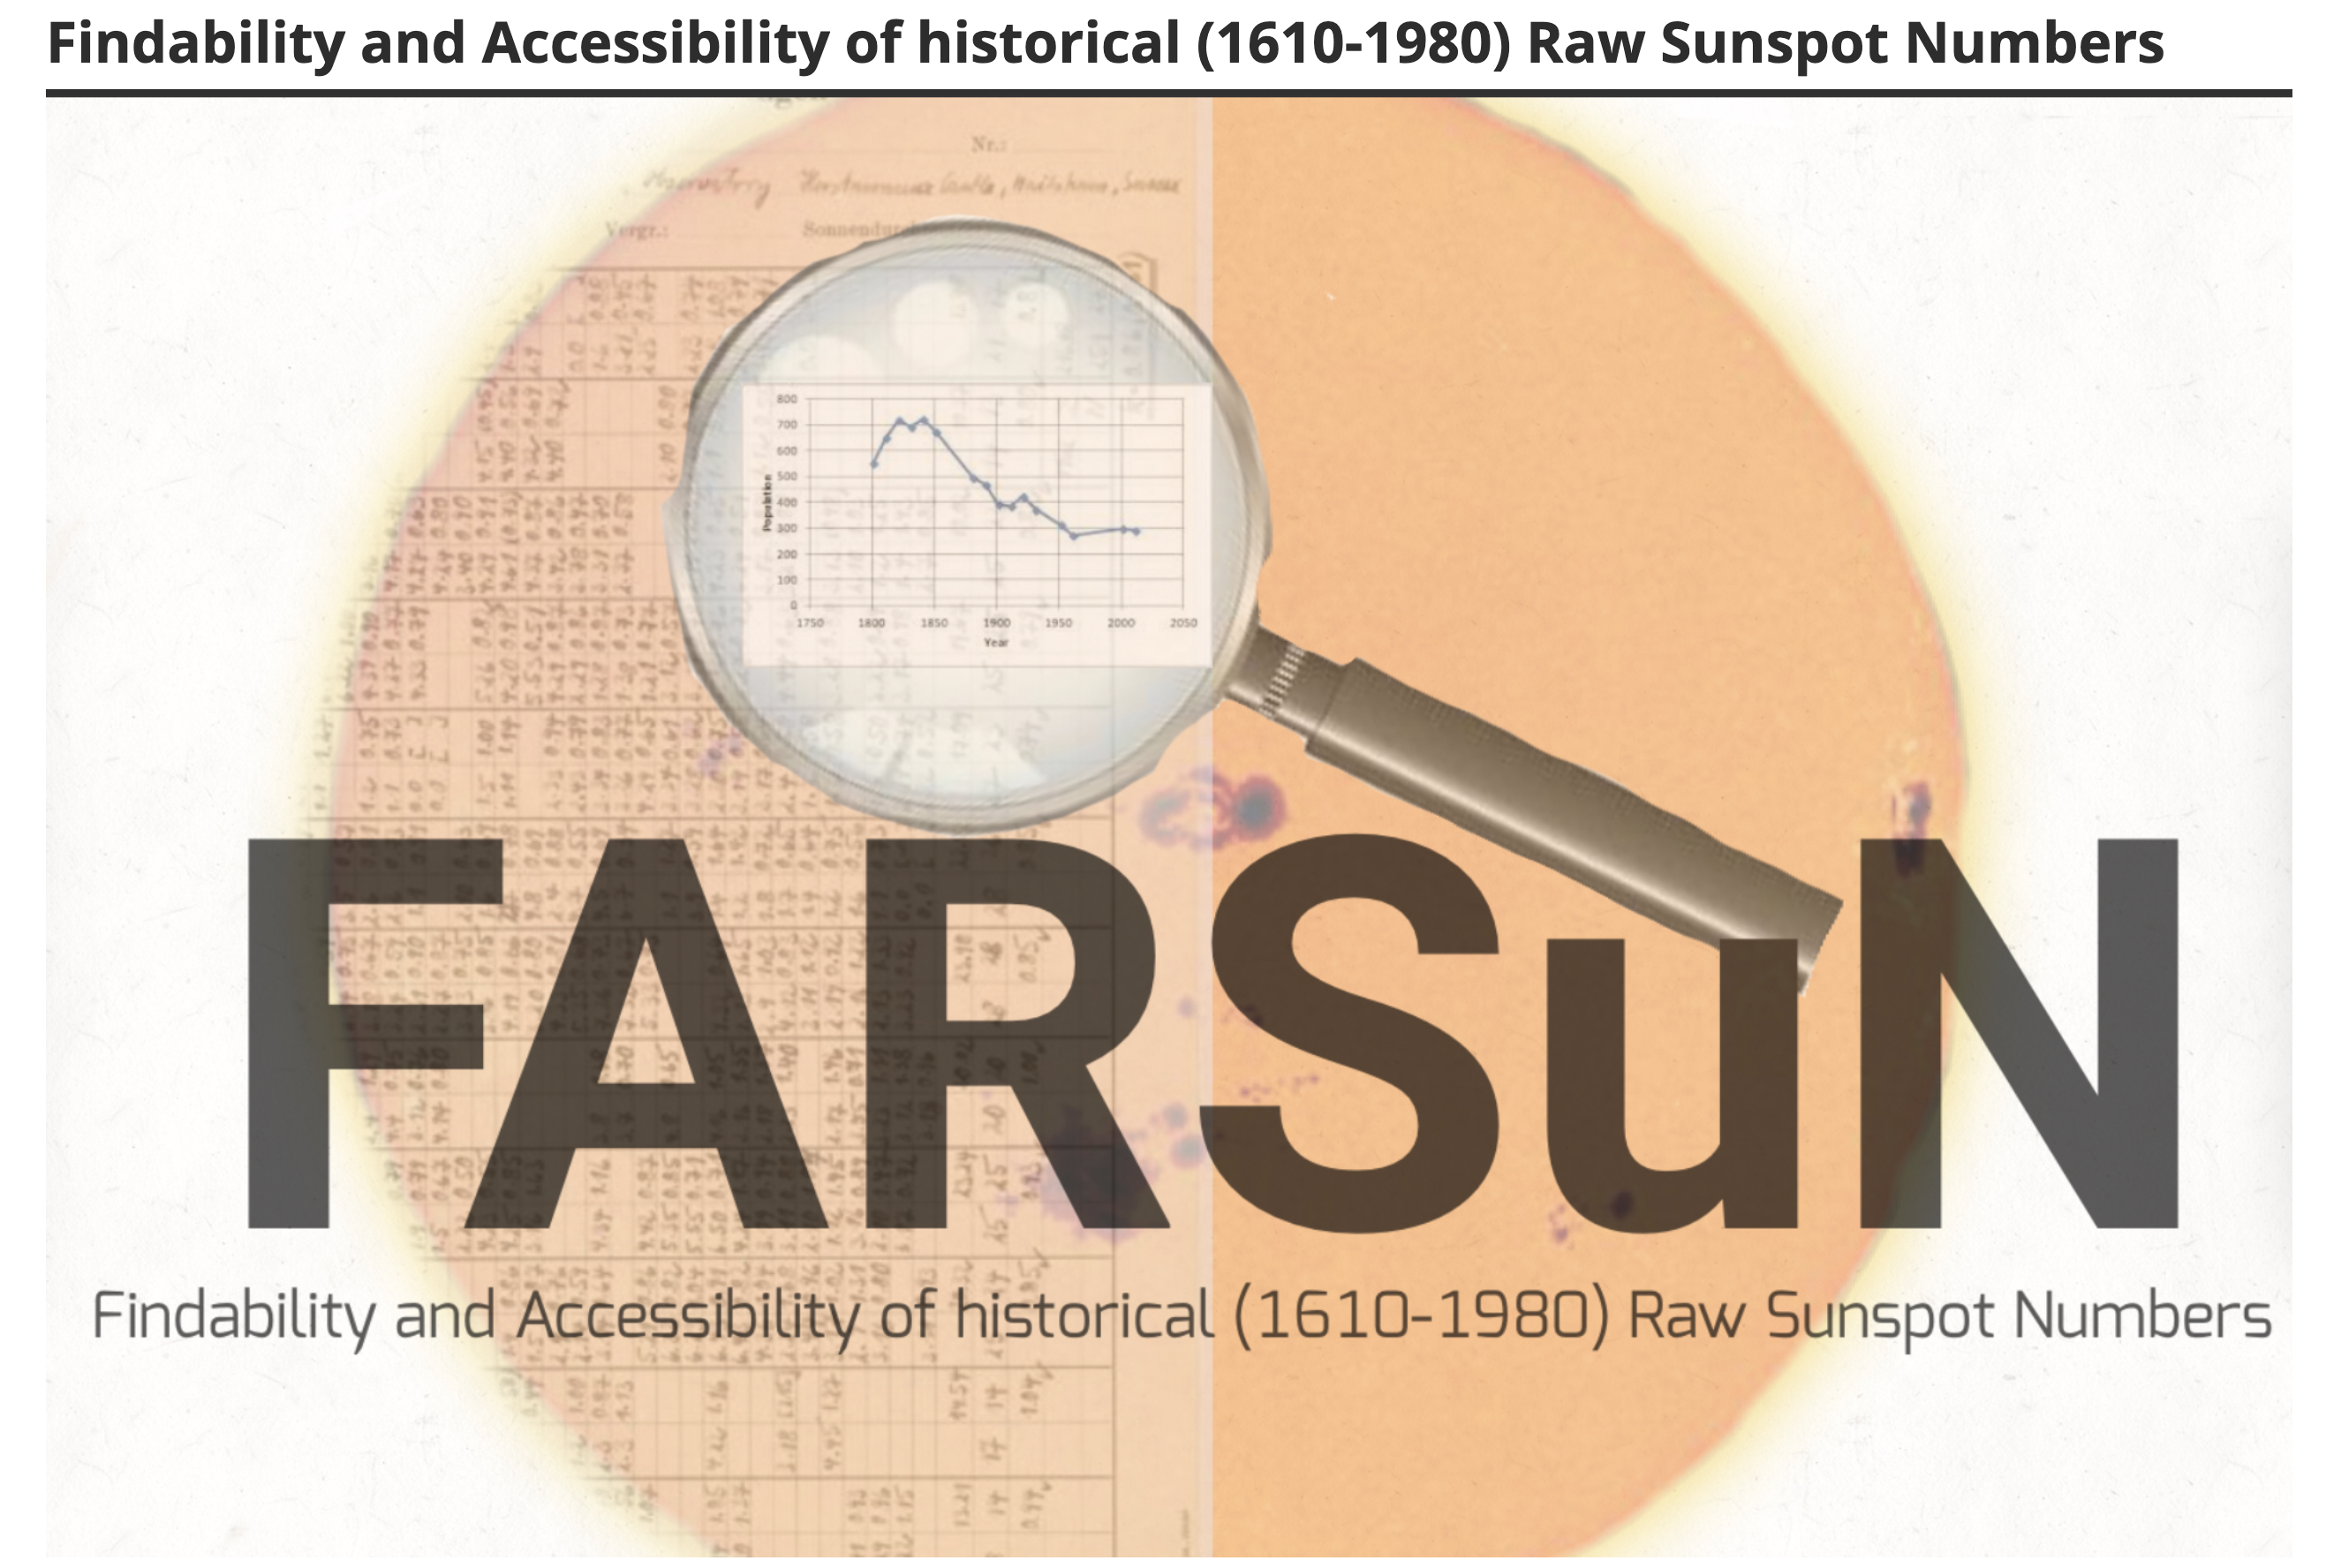
\includegraphics[height=5cm, keepaspectratio]{../figures/ack_.png}
    };

    % Abstract Info Sticky Note (Rotated)
    \node[anchor=north west, rotate=2] at ($(current page.north west)+(3cm,-10cm)$) {
        \begin{tcolorbox}[
          enhanced,
          colback=yellow!50!white,
          colframe=yellow!60!orange,
          boxrule=1pt,
          arc=0mm,
          drop shadow={opacity=0.3, shadow xshift=2mm, shadow yshift=-2mm},
          width=22cm
        ]
        \centering
        \bfseries\small SH23E-2613* -- 16 Dec 2025, 14:15--17:45\\
        Session: The Future of the International Sunspot Number
        \end{tcolorbox}
    };
\end{tikzpicture}

% --- TITLE ---
\vspace{-1.5cm}
\begin{center}
    \color{white}
    {\fontsize{60}{70}\selectfont \textbf{Reconstruction of the Sunspot Number Series : Gathering Data}}\\[0.6em]
    {\Large \textbf{\textcolor{SolarGold}{Kalugodu Chandrashekhar}\textsuperscript{1}}, L. Lef\`evre\textsuperscript{1}, B. Mampaey\textsuperscript{1}, S. Pavai Valliappan\textsuperscript{1}, H. Hayakawa\textsuperscript{2}, C. Ritter\textsuperscript{3}}\\[0.4em]
    {\normalsize \textsuperscript{1}Royal Observatory of Belgium (ROB), \textsuperscript{2}Nagoya University, \textsuperscript{3}Universit\'e Catholique de Louvain}
\end{center}
\vspace{2.5cm}

% --- COLUMNS ---
\begin{columns}[t,totalwidth=0.98\paperwidth]

% ==================== COLUMN 1 ====================
\begin{column}{0.28\paperwidth}

    \begin{abstractblock}
    \justifying
    The Sunspot Number (SN) is one of the longest continuous records of solar activity. SN V2.0 significantly improved the historical series through targeted recalibrations, but recent studies have shown that some scale changes—such as the 1849 transition—can only be fully understood by returning to the original raw observations.
    
    \textbf{This motivates a complete reconstruction (SN V3.0)} in which uncertainties and calibration steps arise directly from the quality of each dataset rather than from global statistical corrections.
    \end{abstractblock}
    \vspace{0.5em}

    \begin{fancyblock}{Four-Axis Methodology}
    \begin{enumerate}
      \item \textbf{Gather Sources}: Track down dispersed observing logs (Wolf's \emph{Mittheilungen}, Z\"urich tables, Gruithuisen manuscripts, Adams drawings) and capture provenance metadata.
      \item \textbf{Process Data}: Use handwriting/OCR engines (Transkribus models) alongside manual double-keying for fragile entries.
      \item \textbf{Validate \& Standardize}: Reconcile aliases, observer IDs, and calendars; model group/spot counting behaviour to derive calibration curves.
      \item \textbf{Disseminate}: Publish machine-readable products, APIs, and VO-ready services with versioned uncertainty bundles.
    \end{enumerate}
    \end{fancyblock}

    \begin{fancyblock}{FARSuN Historical Database}
    A sustainable, interoperable reference database ensuring that four centuries of solar observations remain accessible.
    
    \textbf{Present Status}
    \begin{itemize}
        \item Legacy sources integrated for cross-validation and QC.
        \item Automated quality checks detect inconsistencies (e.g., Groups > Spots).
        \item Metadata harmonization for FAIR/VO standards aligned with EPN-TAP.
    \end{itemize}

    \textbf{Next Steps}
    \begin{itemize}
        \item Finalize canonical schema and close remaining legacy mappings.
        \item Scale up digitization (Adams, Gruithuisen, Stark) using HTR.
        \item Expose full dataset through EPN-TAP service.
        \item \textbf{Foundation for SN V3.0 calibration.}
    \end{itemize}
    \end{fancyblock}

    \begin{fancyblock}{Technical Methods}
    \begin{itemize}
      \item \textbf{Dual-mode transcription:} Tailored Transkribus handwriting models plus manual keying.
      \item \textbf{Data hygiene:} Observer alias reconciliation, calendar conversions.
      \item \textbf{Uncertainty modelling:} Propagate observer calibration curves and spotless-day confidence flags.
      \item \textbf{Automation:} Reproducible Python pipelines with checkpoints.
    \end{itemize}
    \end{fancyblock}
    
    \begin{fancyblock}{Quality Gates}
    \begin{itemize}
      \item \textbf{Two-person verification} for Adams and Gruithuisen counts.
      \item \textbf{Cross-compare} transcriptions with Wolf's \emph{Mittheilungen} and modern indices.
      \item \textbf{Git-tracked pipelines} capture every transformation for audit.
    \end{itemize}
    \end{fancyblock}

\end{column}


% ==================== COLUMN 2 ====================
\begin{column}{0.42\paperwidth}

    \begin{fancyblock}{Key Datasets: The Core Collection}
    
    % --- Dataset 1 ---
    \datasetheader{Mittheilungen Dataset (1610--1945)}{CodeGreen}
    
    \begin{columns}
        \begin{column}{0.45\linewidth}
        The \emph{Mittheilungen} journals, compiled by Rudolf Wolf and successors, form the central source of historical sunspot observations (1848--1945) and incorporate earlier material back to 1610.
        
        \vspace{0.5em}
        \textbf{Status:} Fully digitized at ROB.
        \begin{itemize}
            \item Integrated into FARSuN DB.
            \item Refining consistency and observer calibration (Wolf--Wolfer overlap).
        \end{itemize}
        \end{column}
        
        \begin{column}{0.53\linewidth}
            \centering
            % Placeholder for Image
            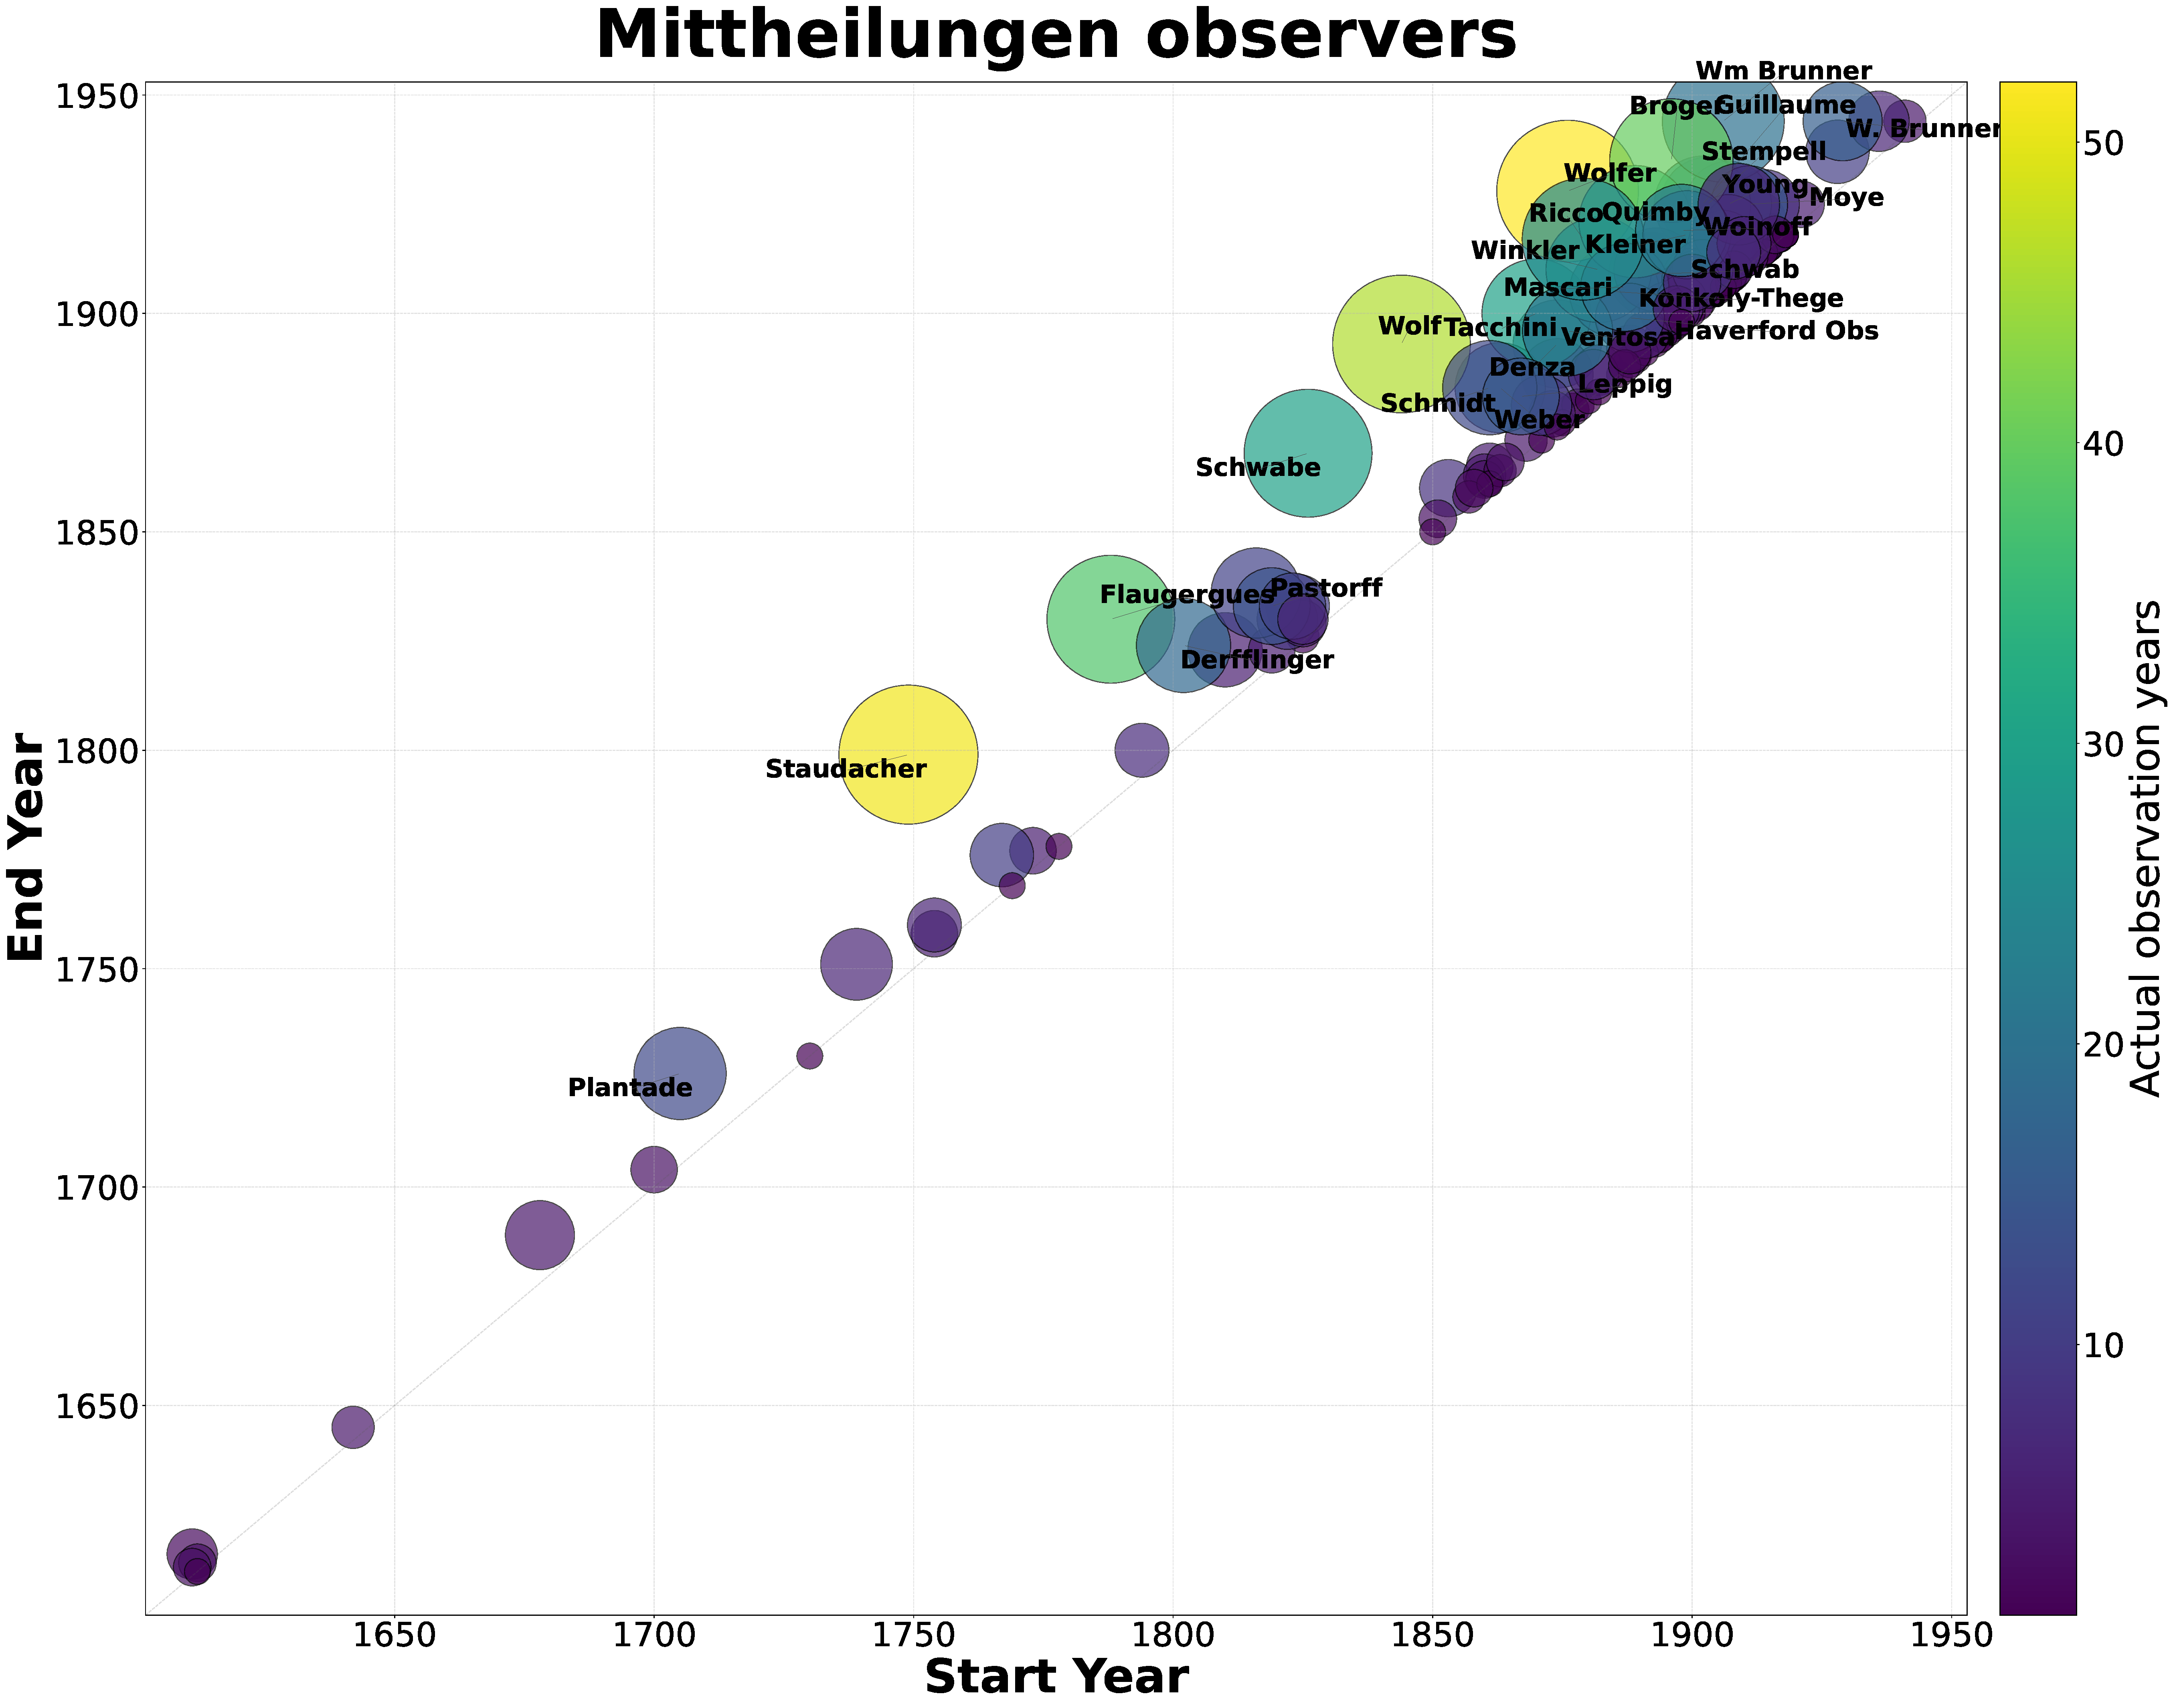
\includegraphics[width=\linewidth]{../figures/mitt_observer_bubble.pdf}
            % \vspace{0.2em}
            % \textit{\footnotesize (Fig: Observer coverage and overlaps)}
        \end{column}
    \end{columns}

    % --- Dataset 2 ---
    \datasetheader{Z\"urich Tables (1945--1979)}{CodeBlue}
    
    The foundational record of daily sunspot number production at Z\"urich.
    
    \textbf{Status:} 95\% of 2,000+ yearly tables digitized.
    \begin{itemize}
        \item Fully digitized for 1945--1979 with detailed metadata completed for 1945--1959.
        \item Quality control and observer metadata harmonisation underway.
    \end{itemize}

    % --- Dataset 3 ---
    \datasetheader{Gruithuisen Data (1817--1849)}{CodeOrange}
    
    Daily sunspot notes, drawings, and weather context in German Kurrent script. Vital early-19th-century coverage.
    
    \begin{columns}
        \begin{column}{0.5\linewidth}
            \centering
            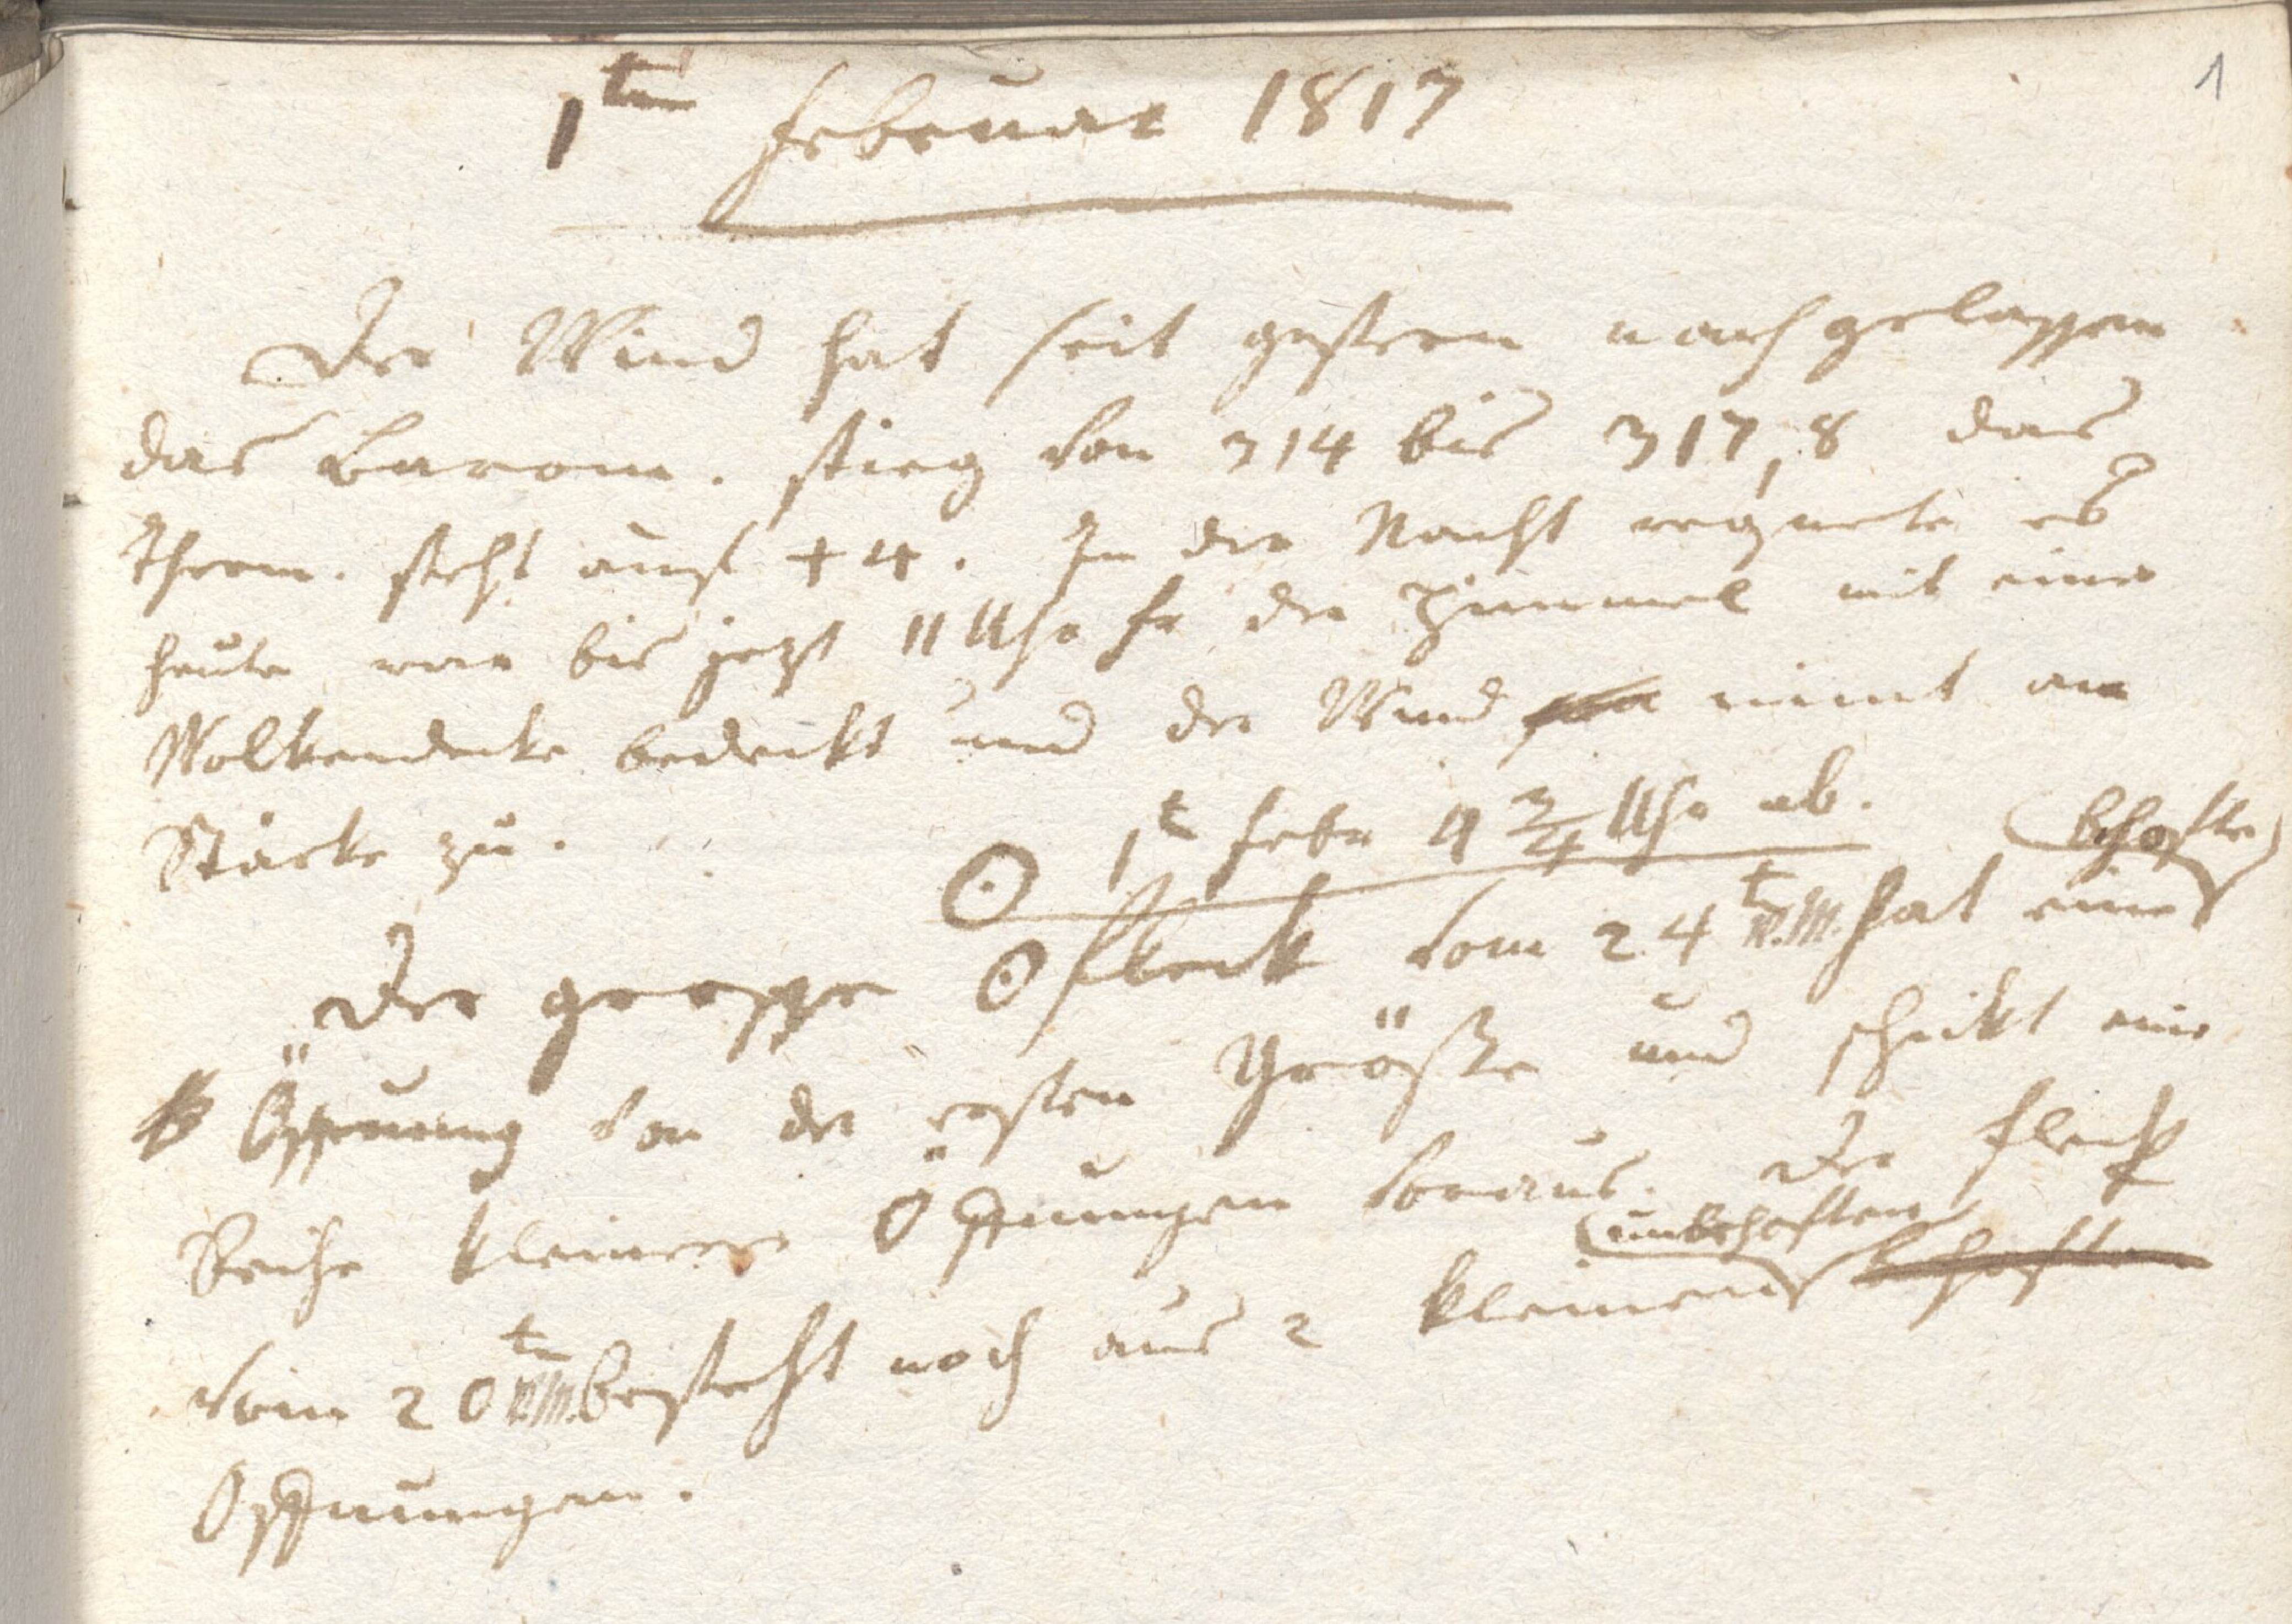
\includegraphics[width=0.95\linewidth]{../figures/Gruithuisen_Sample1.png}
        \end{column}
        \begin{column}{0.5\linewidth}
             \textbf{Status:} Images fully collected.
             \begin{itemize}
                 \item Extraction via bespoke Transkribus models.
                 \item Two-pass QC (survey + counting) in progress.
             \end{itemize}
        \end{column}
    \end{columns}

    % --- Dataset 4 ---
    \datasetheader{C. H. Adams Data (1819--1823)}{CodePurple}
    
    FARSuN has recovered 338 full-disk drawings and 1,056 daily entries.
    \begin{itemize}
        \item Dense coverage with explicit spotless days.
        \item \textbf{Cross-check:} Spotless tallies matched against Wolf's compilations to anchor early-1800s calibration.
    \end{itemize}
    
    \end{fancyblock}

\end{column}


% ==================== COLUMN 3 ====================
\begin{column}{0.26\paperwidth}

    \begin{fancyblock}{Additional Data Recovery}
    
    \datasetheader{Augustin Stark (1813--1835)}{CodeRed}
    Printed German descriptions of sunspot groups. Preliminary OCR shows good potential; refining QC flags and metadata integration.
    
    \vspace{1em}
    \textbf{Timeline of Data Recovery (Since 2010)}
    \begin{center}
        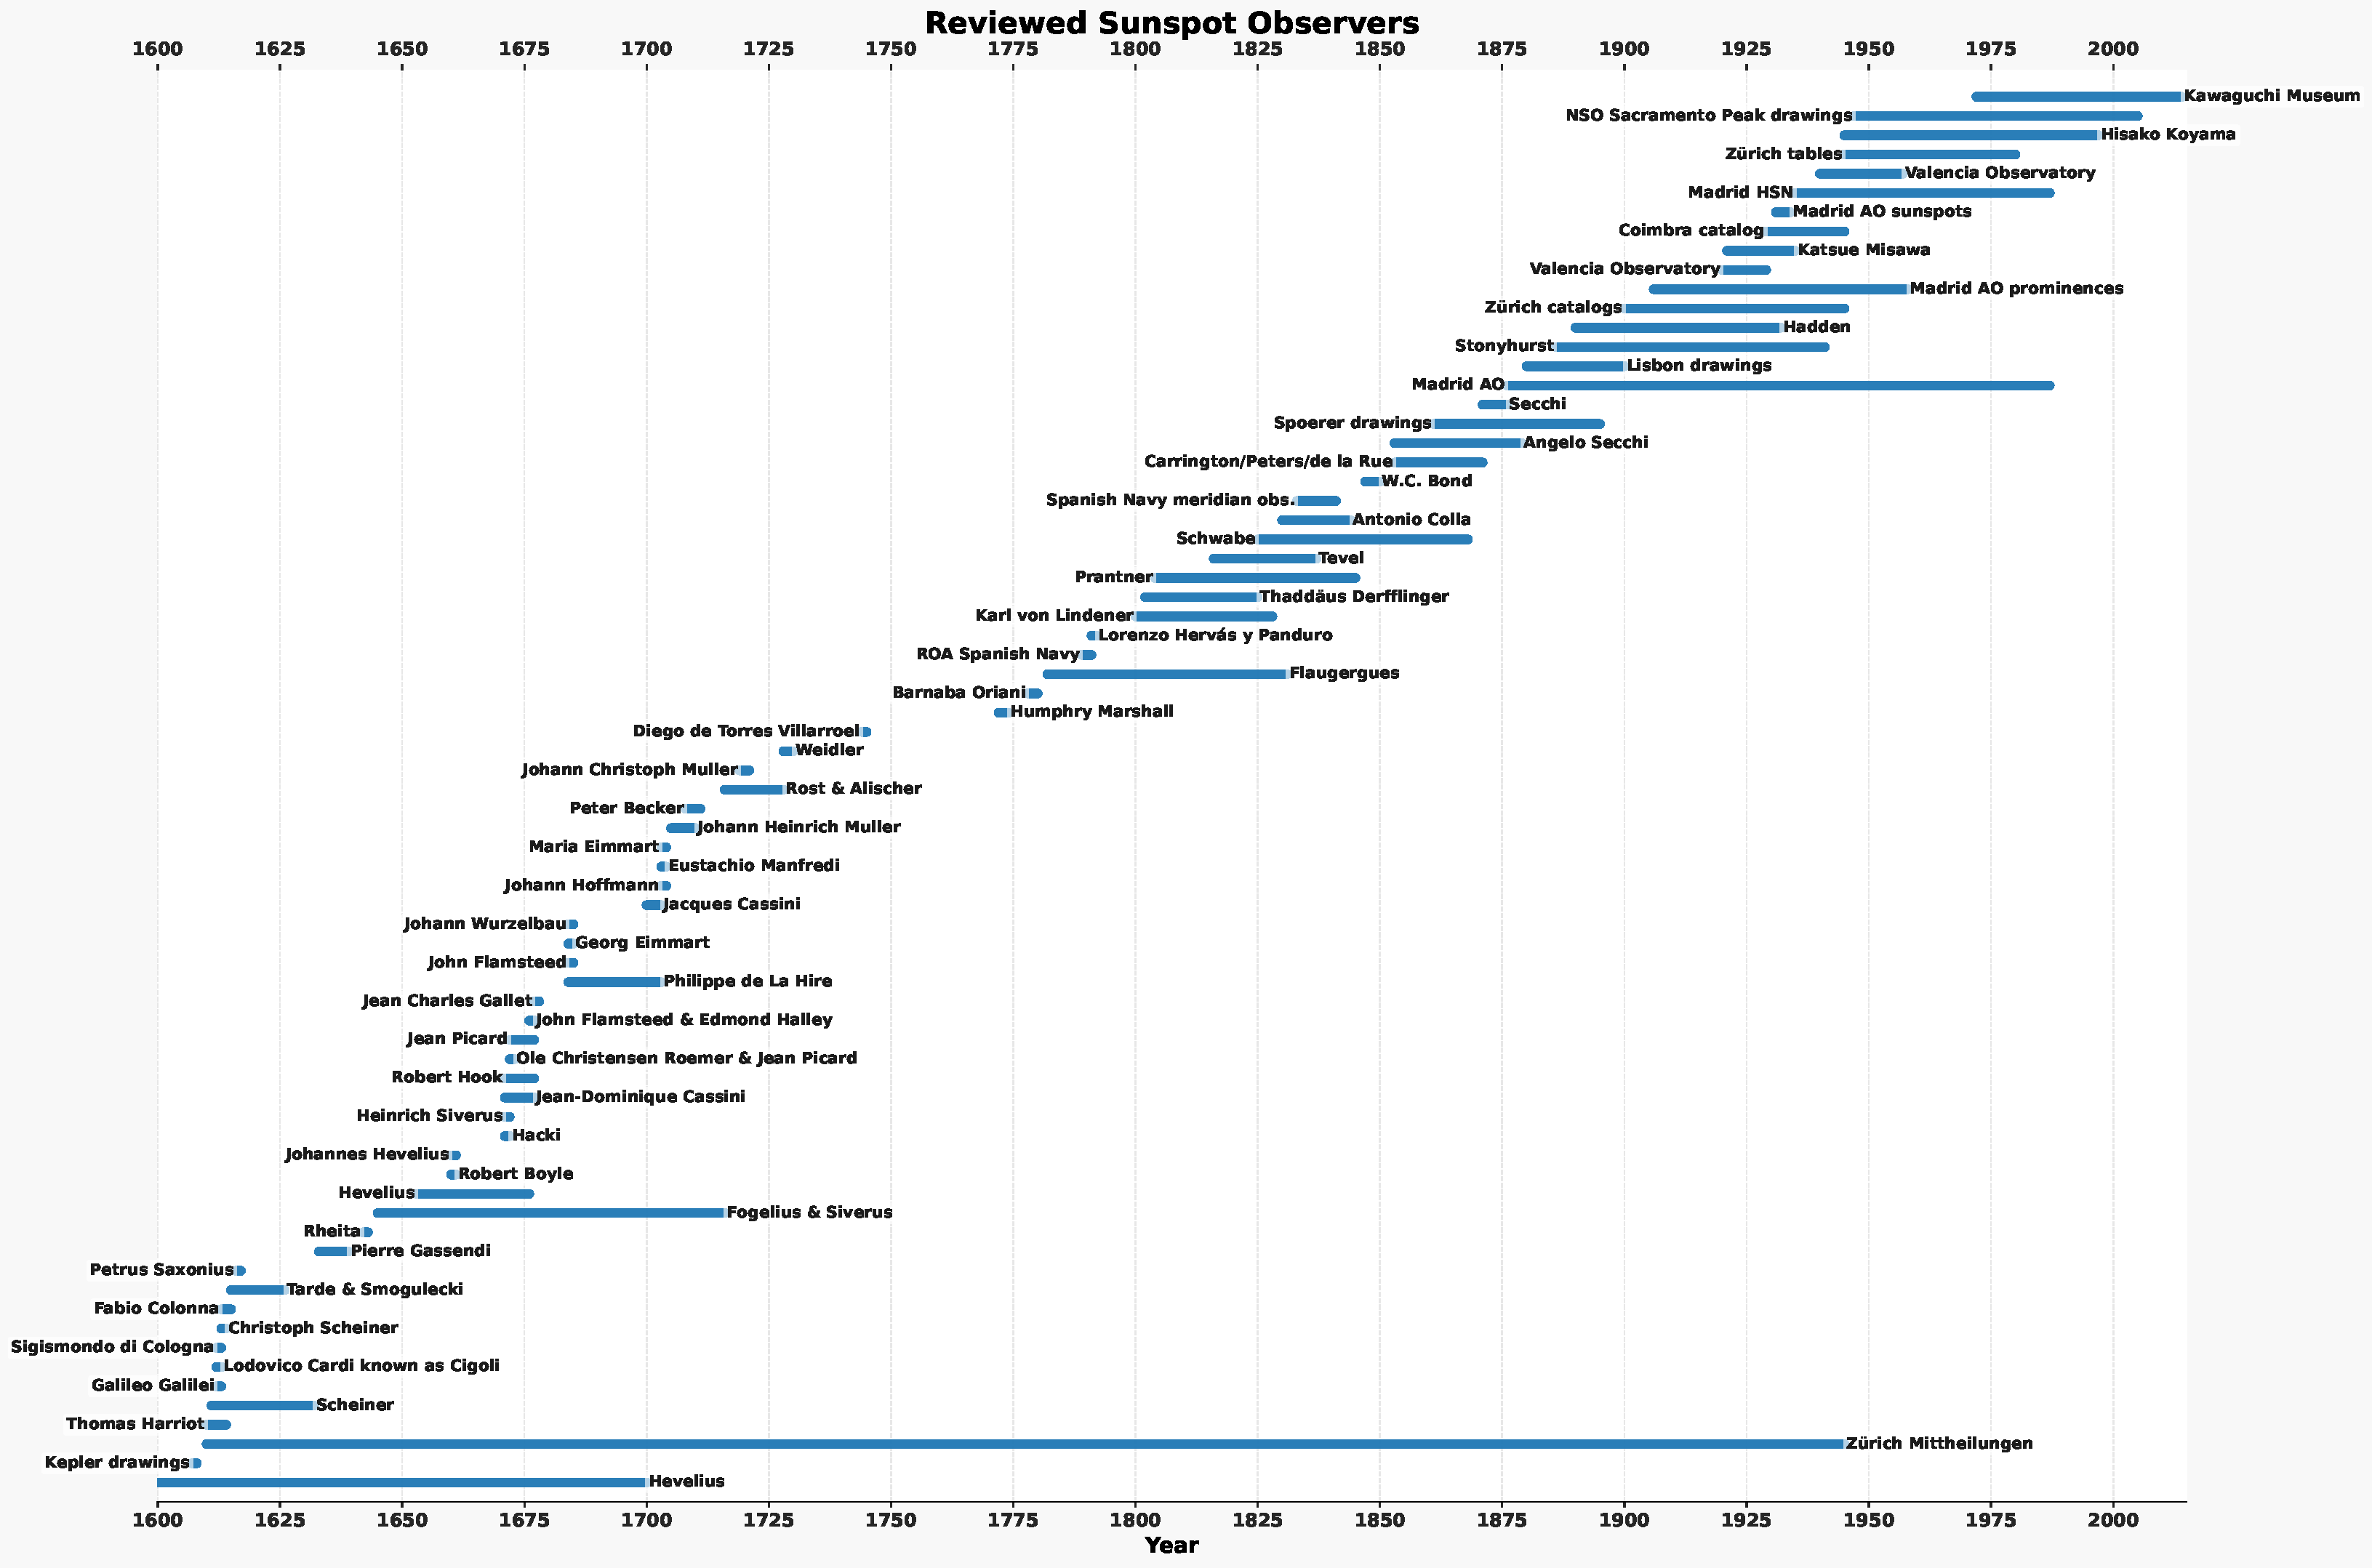
\includegraphics[width=\linewidth]{../figures/reviewed_sources_timeline_merged.pdf}
    \end{center}
    Community efforts (Hayakawa, Arlt, Vaquero, Carrasco) have expanded available raw observations, enabling independent cross-checks.
    \end{fancyblock}

    \begin{fancyblock}{From Raw to SN V3.0}
    \begin{enumerate}
      \item Curate daily counts with provenance-rich metadata.
      \item Solve observer response functions to align scales across centuries.
      \item Aggregate to indices with propagated uncertainties.
      \item Benchmark against SN V2.0 and satellite-era proxies.
    \end{enumerate}
    \end{fancyblock}

    \begin{fancyblock}{Project Challenges}
    \begin{itemize}
      \item Deciphering \emph{Kurrent} manuscripts without losing context.
      \item Harmonising heterogeneous formats (drawings, ledgers).
      \item Quantifying observer bias and spotless-day reporting habits.
      \item Maintaining end-to-end provenance.
    \end{itemize}
    \end{fancyblock}
    
    \begin{fancyblock}{Space Climate Impact}
    \begin{center}
        \calloutcard{CodeGreen}{Citizen Science}{Portal mobilises volunteers to transcribe \emph{Kurrent} \& sustain STEM outreach.}
        \hfill
        \calloutcard{CodeBlue}{Forecasting}{Bias-free SN V3.0 improves solar cycle prediction and operational baselines.}
    \end{center}
    \vspace{0.4em}
    \begin{center}
        \calloutcard{CodeOrange}{Climate Links}{Validated historical forcing refines long-term climate models.}
        \hfill
        \calloutcard{CodePurple}{Open Science}{FAIR-compliant releases with APIs and uncertainty bundles.}
    \end{center}
    \end{fancyblock}

    % QR Code Box
    \begin{tcolorbox}[
        enhanced,
        colback=white,
        colframe=DeepSpace,
        boxrule=2pt,
        arc=4mm,
        sidebyside,
        lefthand width=0.35\linewidth,
        drop shadow
    ]
        
\includegraphics[width=\linewidth]{../docs/figures/qrcode_farsun-poster.png}
        \tcblower
        \textbf{\Large Scan for Data}\\[0.5em]
        For more information on the FARSuN project, datasets, and a digital copy of this poster.\\[0.5em]
        \textbf{Contact:} \url{sidc-support@oma.be}\\
        \textbf{Portal:} \url{https://www.sidc.be/silso/}
    \end{tcolorbox}

\end{column}

\end{columns}

% --- FOOTER ---
\begin{tikzpicture}[remember picture,overlay]
    \fill[DeepSpace] (current page.south west) rectangle ($(current page.south east)+(0,2cm)$);
    \node[white, anchor=center] at ($(current page.south)+(0,1cm)$) {
        \large \textbf{FARSuN}: Findability and Accessibility of Historical Raw Sunspot Numbers
    };
\end{tikzpicture}

\end{frame}
\end{document}
